%!TEX root = BA-Bauer.tex

\subsection{STMicroelectronics CubeMX}
Die Firma STMicroelectronics\textsuperscript{®} bietet für Programmierung der eigenen Mikokontrollern und -porzessoren eine Reihe von kostenloser Software zum Download an. Darunter befindet sich unter anderem die Software CubeMX, die für jeden Mikrocontroller und jedes Entwicklungsboard von STMicroelecronics\textsuperscript{®} verwendet werden kann. Mit der Software können Schnittstellen, Ein und Ausgangspins, Einstellungen der Taktgebung und vieles mehr in einer grafischen Benutzeroberfläche vor der eigentlichen Programmierung konfiguriert werden, was das Durchsuchen des Handbuchs nach den entsprechenden Registern überflüssig macht. CubeMX generiert .c und .h Dateien mit diversen Funktionen für die konfigurierten Schnittstellen und der Hardware. 
Abbildung \ref{fig:CubeMXClock} zeigt die Benutzeroberfläche zur Konfiguration der Taktgebung in CubeMX. 
\begin{figure}[h]
	\centering
	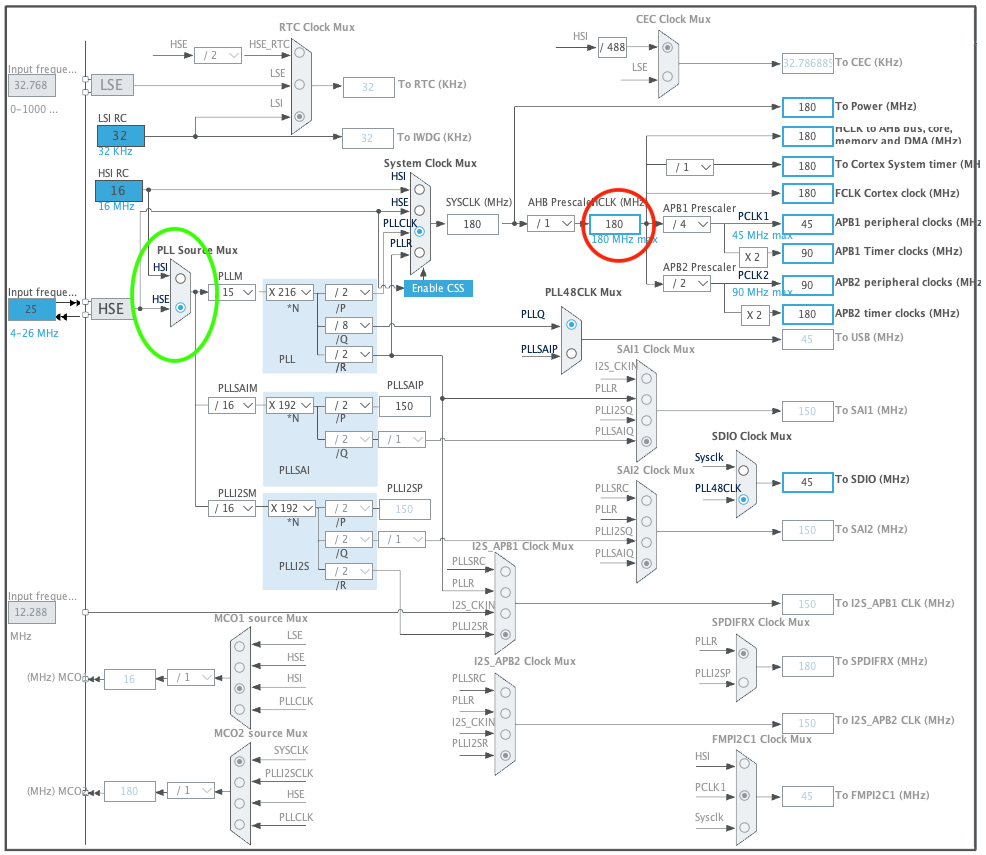
\includegraphics[width=.5\linewidth]{CubeMX-clock-mark}
	\caption{CubeMX Clock Configuration}
	\label{fig:CubeMXClock}
\end{figure}
Die Oberfläche ist nach der Flussrichtung der Taktsignale durch die Parameter und Umschalter angeordnet. Auf der linken Seite finden sich die Oszillatoren, dessen Frequenz durch die in der Mitte befindlichen Parameter und Umschalter geteilt oder multipliziert werden kann. Auf der rechten Seite befinden sich die ausgehenden Taktfrequenzen für die einzelnen Schnittstellen. Um den externen Hochfrequenzoszillator zu verwenden, wird im grün markierten Bereich der $HSE$ Umschalter aktiviert und die Frequenz des Oszillators links neben dem grün markierten Bereich einegeben. Damit der Mikrocontroller mit der maximalen Taktfrequen von 180\,MHz arbeitet wird das rot markierte Feld mit 180 beschrieben. CubeMX berechnet alle Parameter und Umschalter um die gewählte Taktfrequenz des Mikrocontrollers und der verwendeten Schnittstellen zu erreichen. Anhand der großen Anzahl an Variablen ist das Einstellen der Parameter und Umschalter per Hand nur mit sehr großem Aufwand zu bewerkstelligen. CubeMX unterstützt den Prozess des Programmierens auch in der Konfiguration von Schnittstellen. Der in dieser Arbeit verwendete STM32F446ZE Mikrokontroller besitzt 20 Schnittstellen welche ohne CubeMX einzeln durch das Beschreiben von Registern konfiguriert werden müssten. Mit CubeMX können diese Schnittstellen mithilfe einer grafischen Oberfläche eingestellt werden. Zudem schlägt die Software verwendbare Pins zu den jeweiligen Schnittstellen vor, welche durch die Zuweisung an einem virtuellen Mikrocontroller der Schnittstelle zugeordnet werden kann. Die Pins des Mikrocontrollers besitzen unter Umständen mehrere Funktionen gleichzeitig, können jedoch nur von einer Schnittstelle parallel verwendet werden.  Solche Überschneidungen werden von CubeMX erkannt und können manuell durch die Zuweisung eines anderen noch verfügbaren Pins behoben werden.
%\begin{figure}[h] 
%	\centering
%	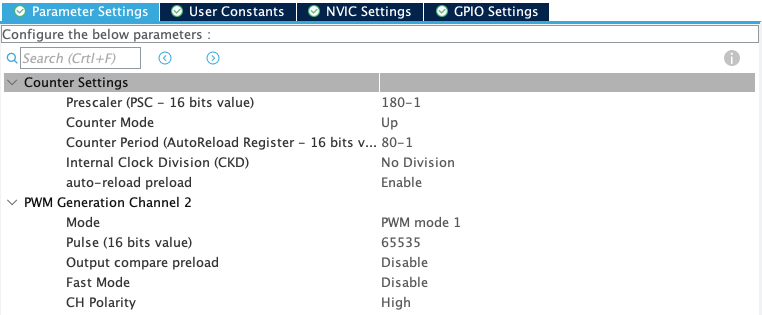
\includegraphics[width=.5\linewidth]{CubeMX-timerconfig}
%	\caption{CubeMX Beispiel Schnittstellenkonfiguration Timer}
%	\label{fig:CubeMXTimer}
%\end{figure}
%Schnittstellenzuweisung der Pins
%Funktionen der Pins
%Interrupts etc. aktivieren
%Koniguration der Schnittstellen
%HAL?!?!